\subsection{A priori error estimates}

The need for \textit{h-adaptivity} arises from the inefficiency encountered solving the Poisson problem over sequences of uniform meshes while working with pathological exact solutions such as \eqref{pathological_square} and \eqref{pathological_lshape}.

The first step to implement \textit{h-adaptivity} is to evaluate the $\LT$ error on each element and then refine the element with the highest error according to a specific refinement strategy.

The strategy of choice can be outlined as follows:

\begin{enumerate}
    \item For polygons with $N_e \leq 4$, the refiner adds a single node at the polygon's centroid and then connects each edge's midpoint to this new node, creating $N_e$ new quadrilaterals.
    \item For polygons with $N_e > 4$, the refiner adds $N_e$ new nodes at the midpoints of the segments connecting the polygon's centroid to the midpoints of its edges. The refiner then connects these points to form quadrilaterals along the polygon's edges and creates a new smaller polygon by connecting all the new internal nodes.
\end{enumerate}

Meshes and error trends in the following pages.

\newpage
\subsubsection{Meshes}

\begin{figure}[!ht]
	\centering
	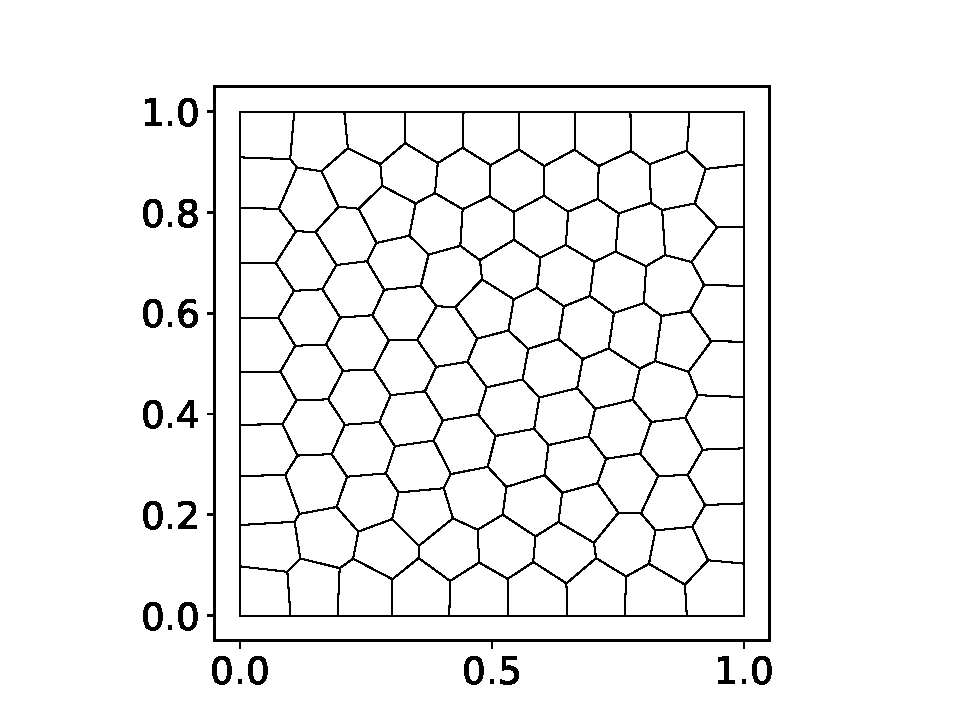
\includegraphics[trim=0cm 0.5cm 0cm 0.5cm, clip, width=5.5cm]{square_100.pdf}
    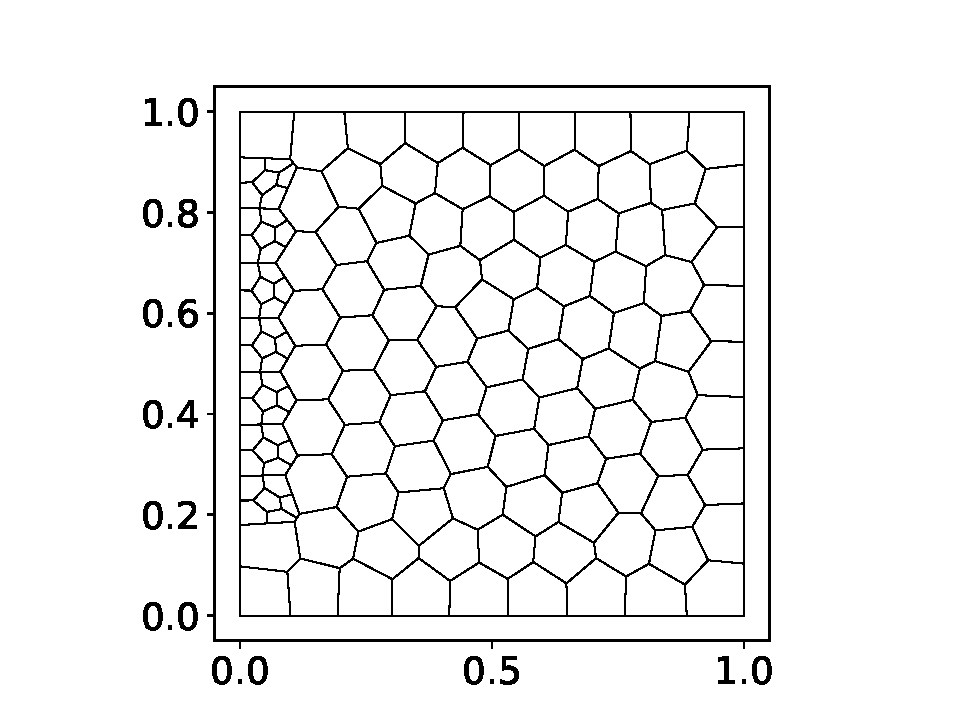
\includegraphics[trim=0cm 0.5cm 0cm 0.5cm, clip, width=5.5cm]{square_100_h1.pdf}
    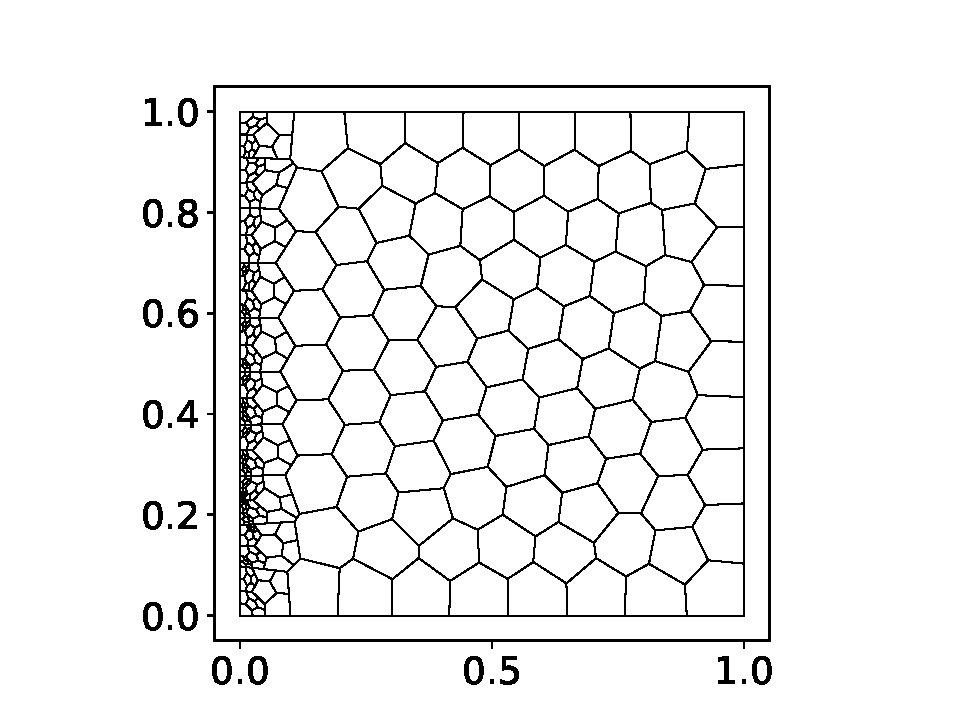
\includegraphics[trim=0cm 0.5cm 0cm 0.5cm, clip, width=5.5cm]{square_100_h2.pdf}
	\caption{Square mesh after 0, 1 and 3 refinements.}
\end{figure}

\begin{figure}[!ht]
	\centering
	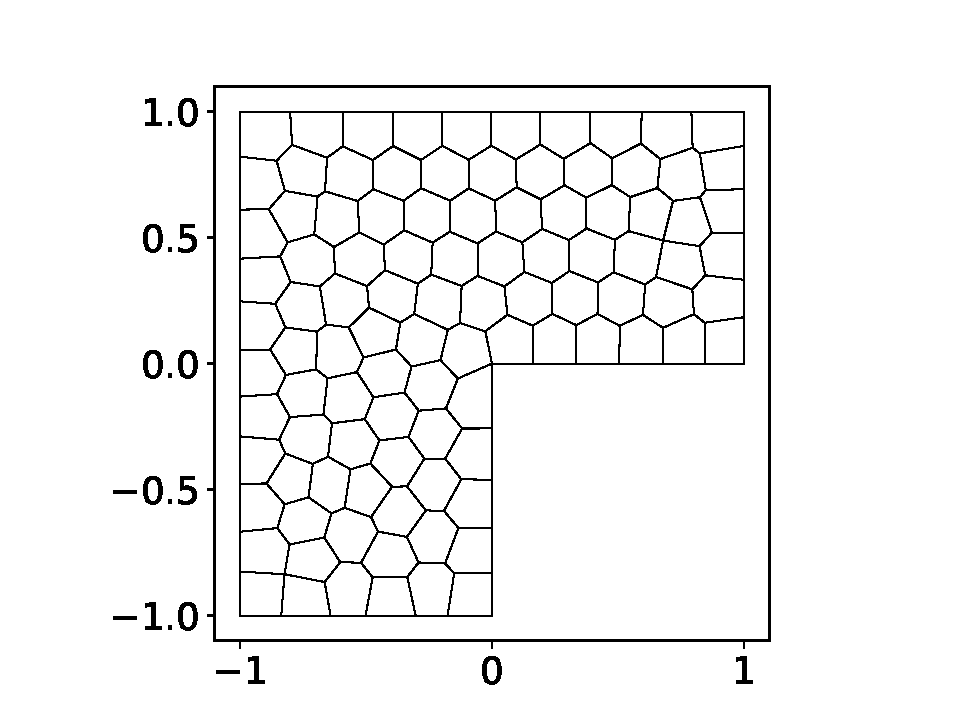
\includegraphics[trim=0cm 0.5cm 0cm 0.5cm, clip, width=5.5cm]{lshape_100.pdf}
    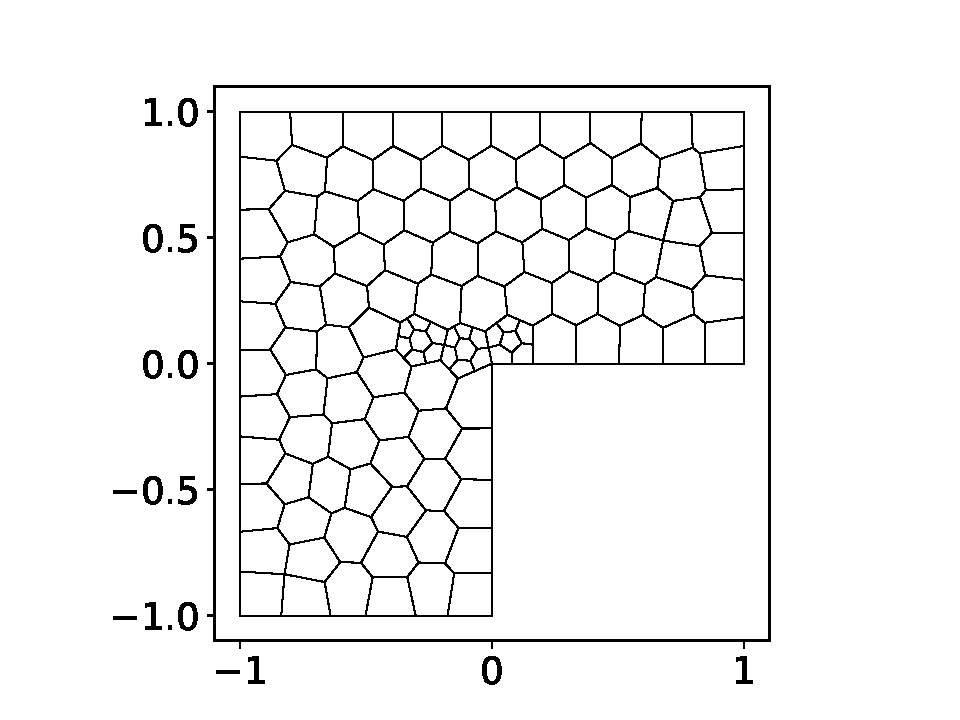
\includegraphics[trim=0cm 0.5cm 0cm 0.5cm, clip, width=5.5cm]{lshape_100_h1.pdf}
    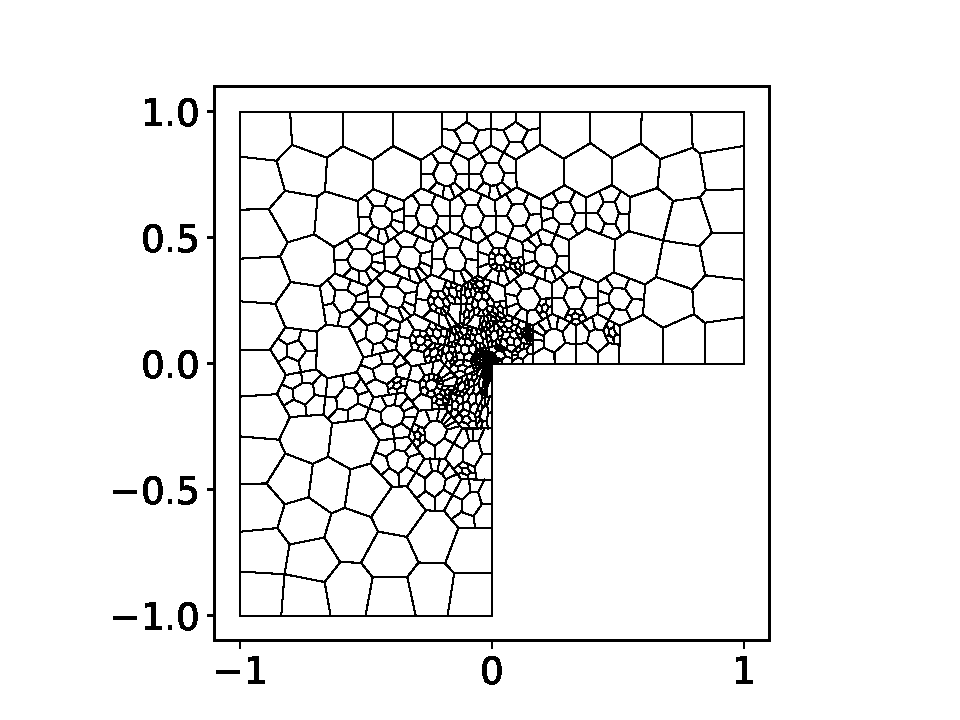
\includegraphics[trim=0cm 0.5cm 0cm 0.5cm, clip, width=5.5cm]{lshape_100_h2.pdf}
	\caption{L-shaped mesh after 0, 1 and 3 refinements.}
\end{figure}

\newpage
\subsubsection{Errors}

\begin{figure}[!ht]
	\centering
	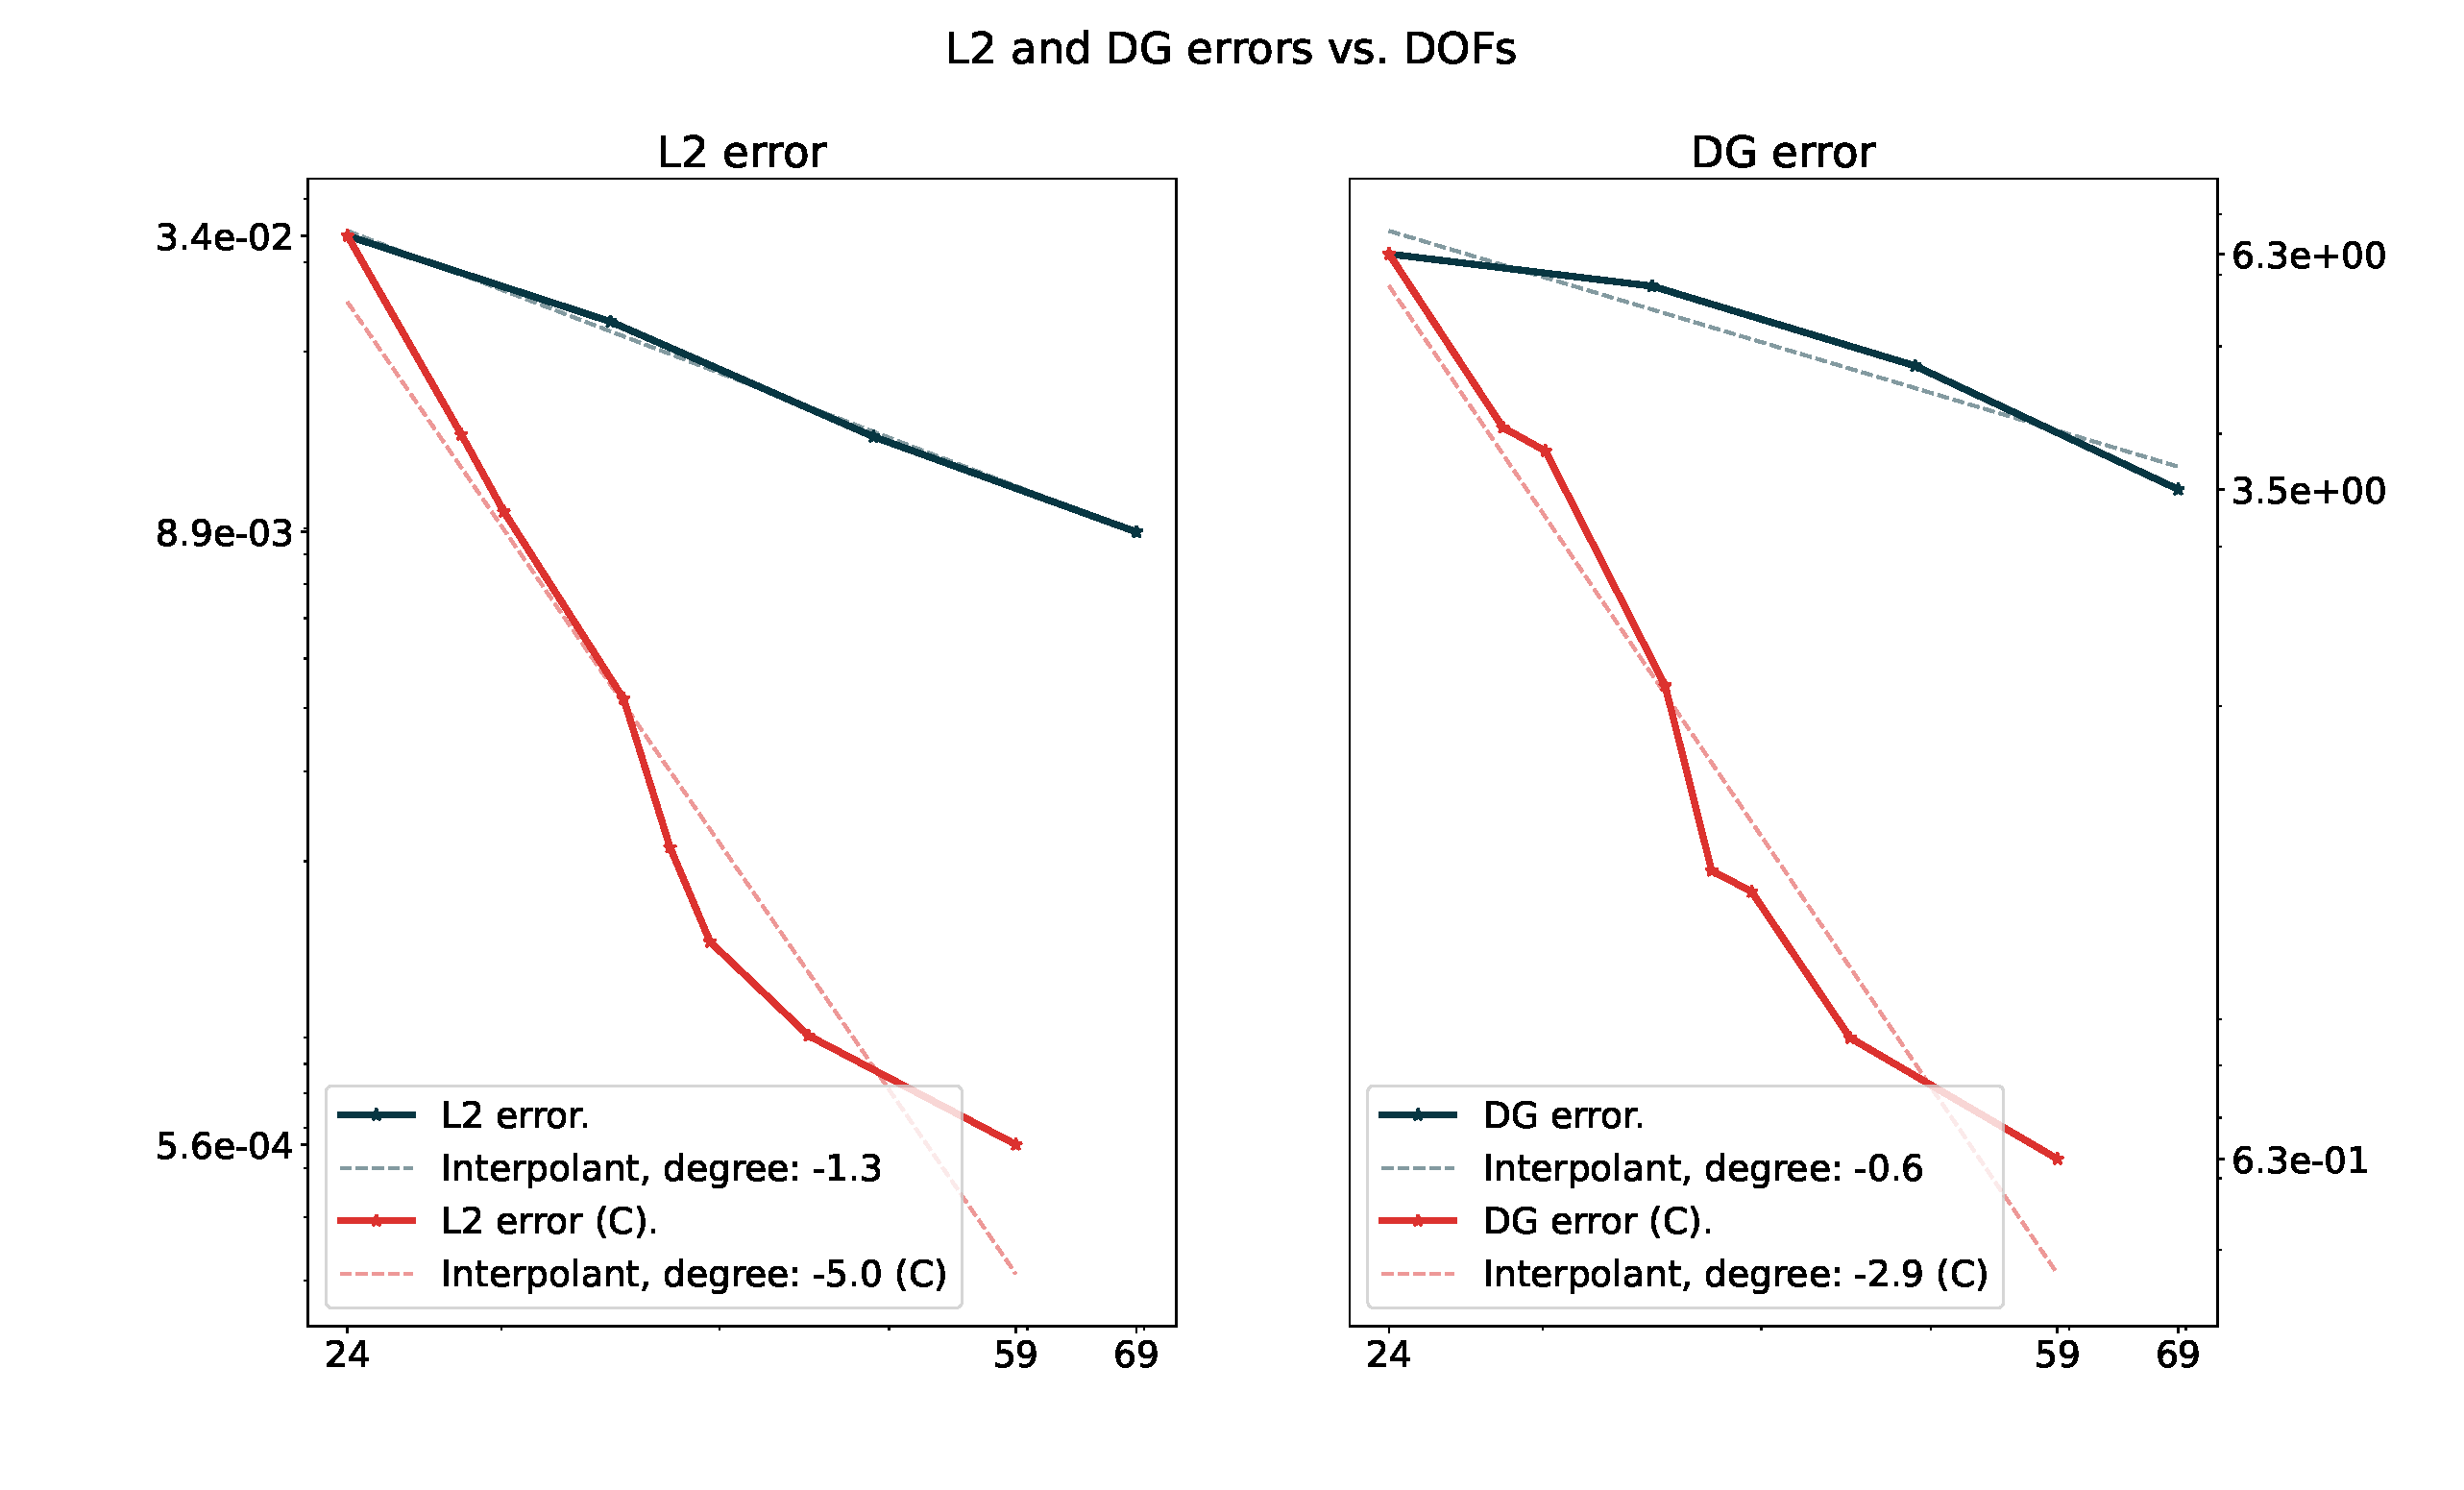
\includegraphics[trim=0cm 0.5cm 0cm 2cm, clip, width=16cm]{square_h.pdf}
    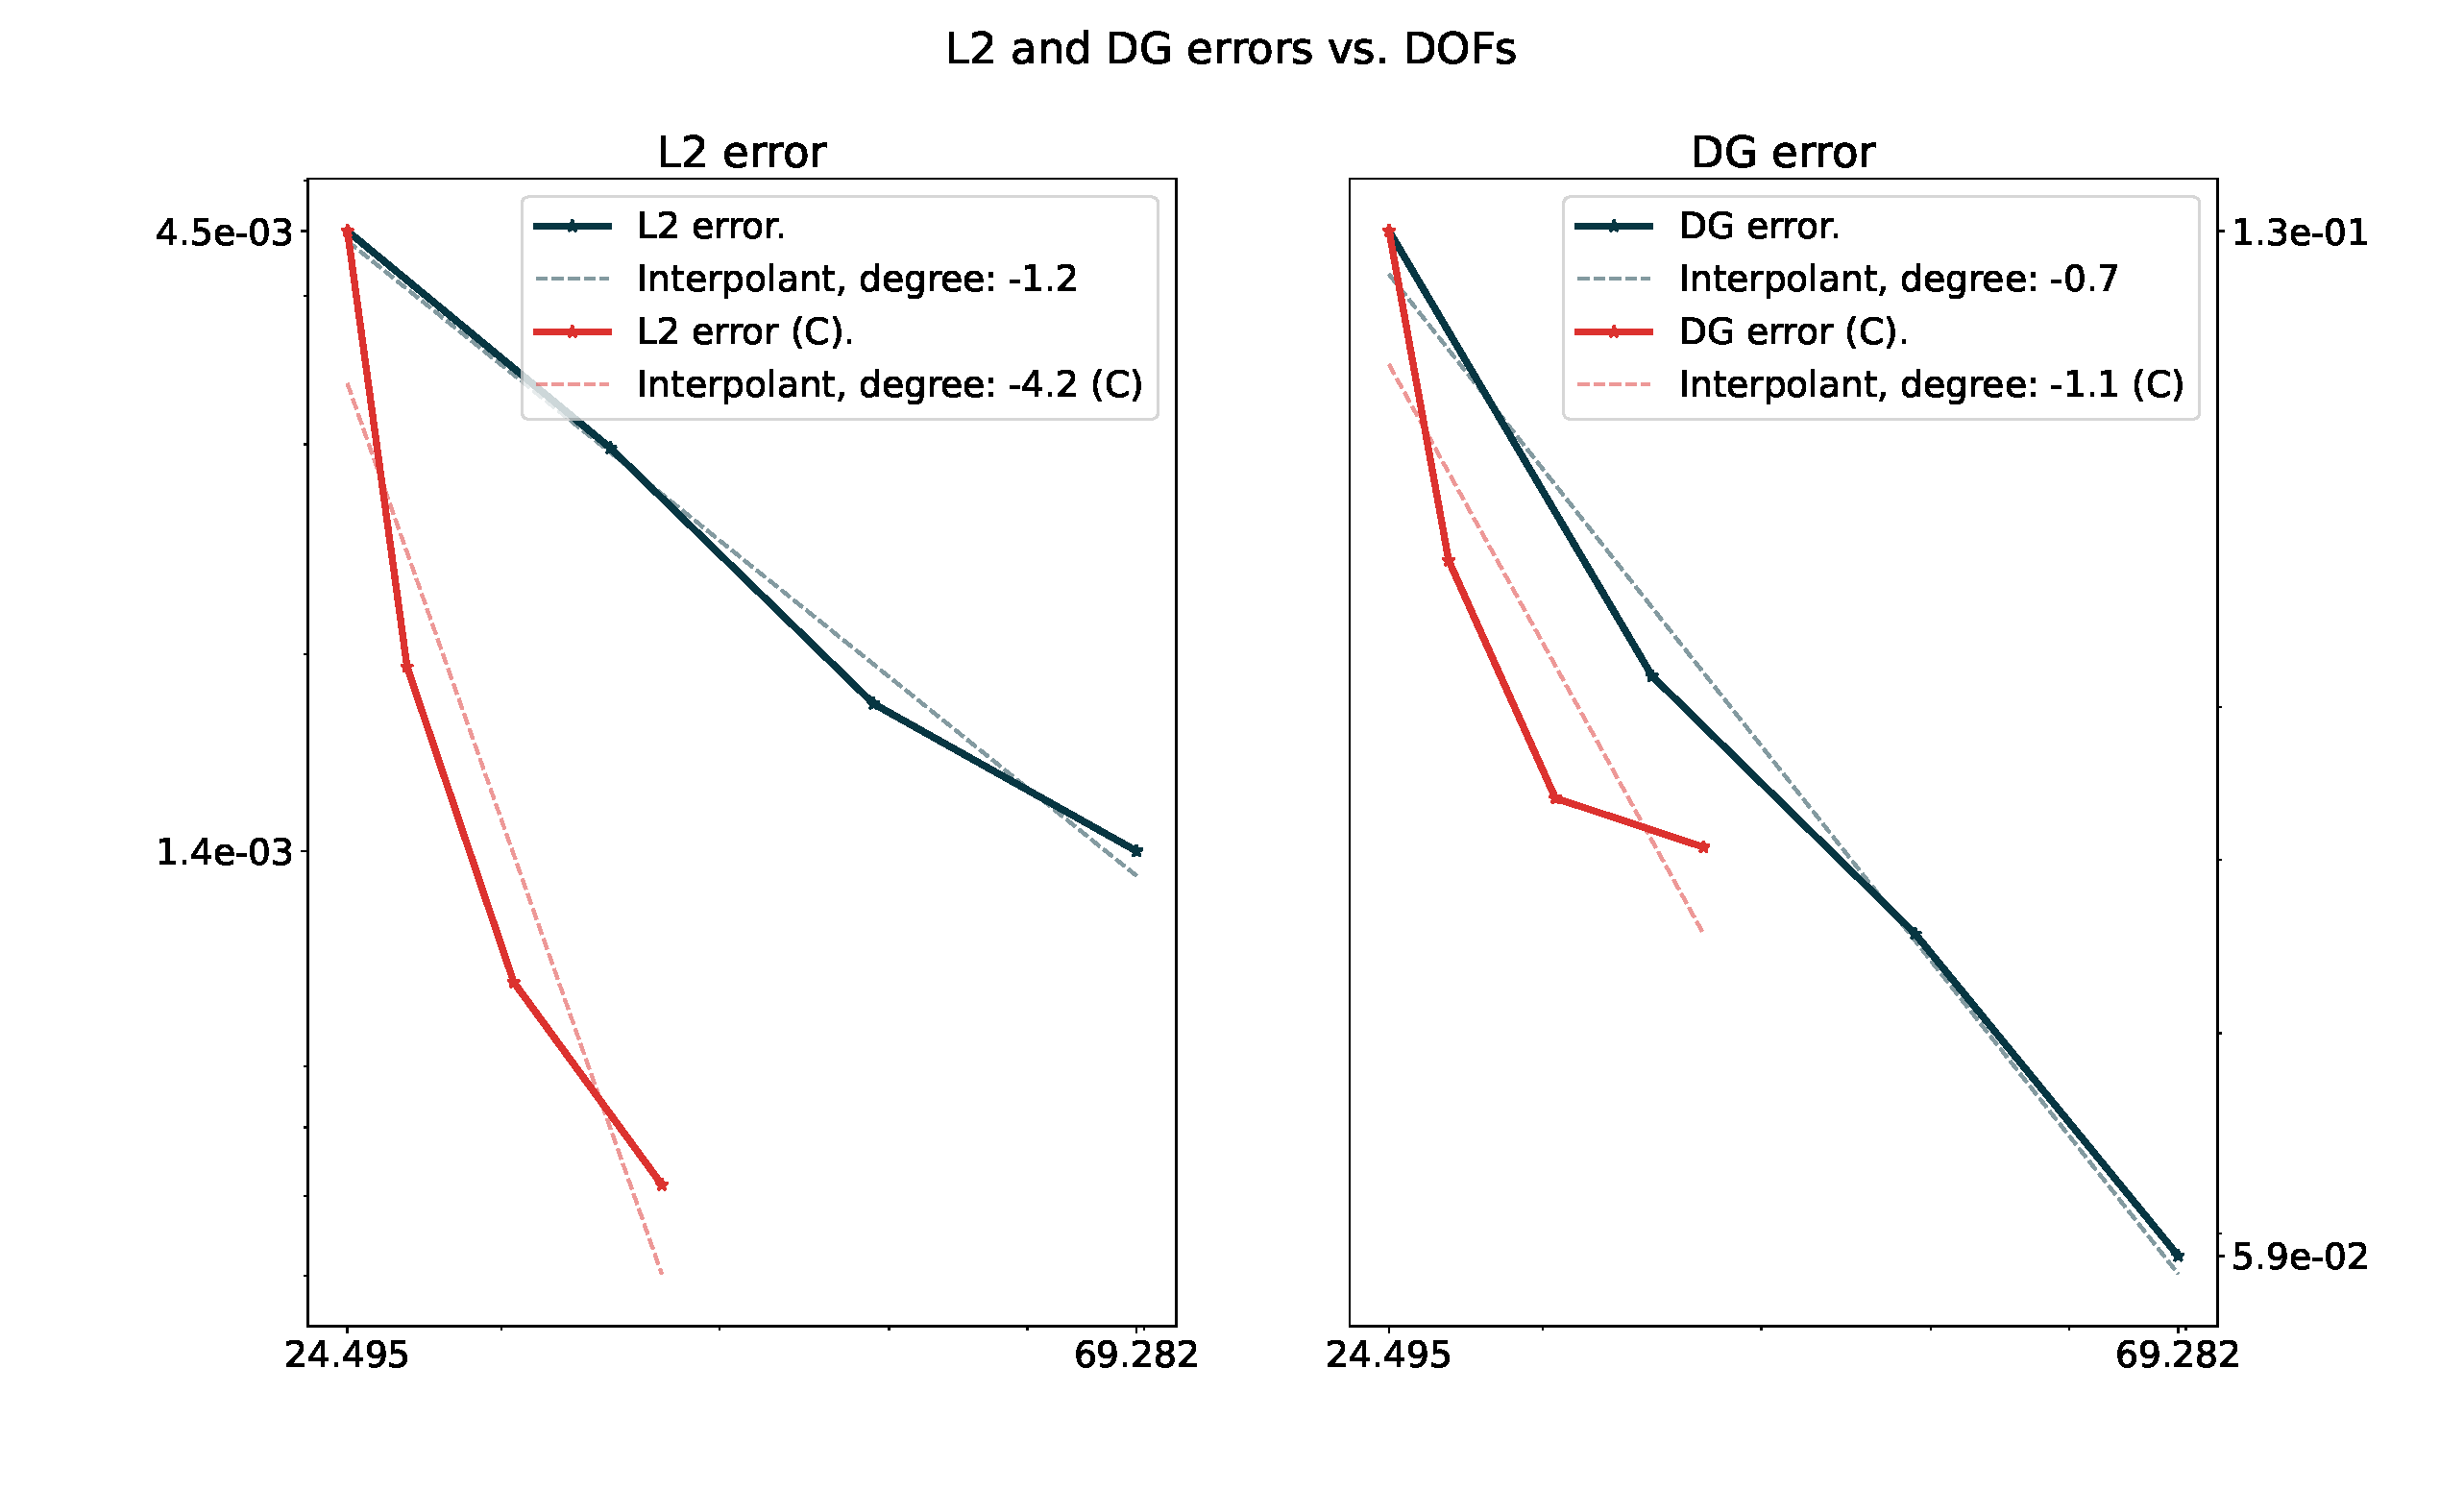
\includegraphics[trim=0cm 0.5cm 0cm 2cm, clip, width=16cm]{lshape_h.pdf}
	\caption{Comparison of $\LT$ and DG errors versus $\text{DOFs}^{1/2}$ between a sequence of uniform meshes and \textit{h-adaptively} refined meshes over a square domain (top) and an L-shaped domain (bottom), with $k = 2$ and $N \in \{100, 200, 400, 800\}$.}
\end{figure}

\newpage
\subsection{A code snippet}

